% Chapter 4 -- Implementation and Experimental Setup
% Status: basic draft. All numbers via macros/tables. Pending: nothing blocking.
\chapter{Implementation and Experimental Setup}
\label{ch:setup}

\section{Dataset}
\label{sec:setup-data}

MovieLens 1M \cite{harper2015movielens} contains \DsRatings{} ratings by \DsUsers{} users on
\DsItems{} films; every user has at least \DsMinRatings{} ratings. All ratings are treated as
implicit positives, as in NCF and PFedRec. Table~\ref{tab:dataset} summarises the data. Users are
grouped by their number of \emph{training} interactions into sparse $[0, 30)$, medium $[30,
100)$ and dense $[100, \infty)$; the groups are fixed by the split and shared by every method.
Two properties of the data constrain the interpretation. The ``sparse'' group is not a cold-start
group: its users have between 19 and 29 training interactions, and only \DsExactlyTwenty{} users
have the minimum of 20 ratings, so the sparse-user penalty of the adaptive rule
(Section~\ref{sec:method-adaptive}), which fires below 20 interactions, affects at most those
users. And the data are dense by recommendation standards (\DsDensity\%), which favours methods
with a shared item table.

\begin{table}[htbp]
  \caption{MovieLens 1M statistics and user groups.}
  \label{tab:dataset}
  \centering\small
  \fittable{% AUTO-GENERATED by thesis/scripts/build_assets.py -- do not edit by hand.
% MovieLens 1M statistics from data/ml-1m/ratings.dat; groups by training count
\begin{tabular}{lr}
\toprule
Statistic & Value \\
\midrule
Users (= clients) & 6,040 \\
Items & 3,706 \\
Ratings (all treated as implicit positives) & 1,000,209 \\
Density & 4.47\% \\
Ratings per user: min / median / mean / max & 20 / 96 / 165.6 / 2,314 \\
Training interactions per user (one test item held out) & ratings $-$ 1 \\
Sparse users ($[0, 30)$ training interactions) & 809 \\
Medium users ($[30, 100)$) & 2,322 \\
Dense users ($[100, \infty)$) & 2,909 \\
\bottomrule
\end{tabular}
}
\end{table}

\section{Evaluation Protocol}
\label{sec:setup-protocol}

The protocol was locked before the cited runs and is identical for the four methods.
\begin{itemize}[leftmargin=2em]
  \item \textbf{Partition.} Natural, one user per client, $N=\NClients$ clients.
  \item \textbf{Split.} Leave-one-out: the latest interaction of each user is the test item;
        there is no validation item (Section~\ref{sec:setup-validity} reports the consequence).
  \item \textbf{Candidates.} The test item plus 99 items the user never interacted with,
        sampled once from a fixed seed and stored with the split, so that every method and every
        re-scoring variant ranks the same 100 items for a given user.
  \item \textbf{Metrics.} \ndcg{} (primary), \hr{} and \mrr{} over the 100 candidates,
        averaged over all \DsUsers{} users and within the three groups.
  \item \textbf{Federation.} $C=\ParticipationC$ clients sampled uniformly per round,
        $R=\NRounds$ rounds, $K=1$ local epoch, seed \Seed{} for all samplers.
  \item \textbf{Checkpoint rule.} The in-loop metric of the sampled clients is tracked every
        round; the global parameters of the best round are restored and the \emph{full
        population} is scored once with them (the ``D-06'' evaluation). The reported number is
        that full-population score.
  \item \textbf{Negative sampling for training.} Negatives are drawn from the items the user has
        not trained on, through a shared exclusion table; in the federated runs this table also
        excludes the test item, as released FedRec code does. The post-tuning experiment runs
        both conventions (Section~\ref{sec:method-posttune}).
\end{itemize}

\section{Implementation}
\label{sec:setup-impl}

The four methods are four packages on Flower \cite{beutel2020flower} and PyTorch
\cite{paszke2019pytorch} that share one foundation library for the split, the exclusion table,
the user groups, the candidate sampler, the metrics, the mode profiles and the result manifest.
Private parameters are stored per client in an on-disk cache keyed by the run identifier, loaded
at the start of a participation and saved at its end; the same cache is read by the final
full-population evaluation and by the offline re-scoring tool. Each run writes a
\code{results.json} with the full configuration, the per-round in-loop metrics, the client
selection of every round, the best round and the final metrics, and an
\code{EVAL\_VALIDITY.json} sidecar that records whether the evaluation code contained the fixes
of Section~\ref{sec:setup-validity}. Table~\ref{tab:runs} lists the cited runs.

\begin{table}[htbp]
  \caption{The cited runs. $^{\dagger}$Wall-clock time from the run identifier to the result
  timestamp on one RTX 5090 (includes the final full-population evaluation).}
  \label{tab:runs}
  \centering\small
  \fittable{% AUTO-GENERATED by thesis/scripts/build_assets.py -- do not edit by hand.
% run provenance from results.json (_manifest.git_commit, final_metrics.best_round) and EVAL_VALIDITY.json
\begin{tabular}{llllllr}
\toprule
Method & Run & Commit & Best round & Calibration & Validity & Hours$^{\dagger}$ \\
\midrule
Baseline (all-global BPR-MF) & e81518 & 7e0f9b2 & 83 & no & valid & 22 \\
Personalized (split learning) & f18e64 & 9ce092d & 33 & no & valid & 41 \\
PFedRec (+ final calibration) & cf72e0 & 62961dc & 83 & yes & valid & 15 \\
Adaptive (dual-level, $\alpha$ blend) & 869730 & bb67cff & 83 & no & valid & 23 \\
PFedRec (no calibration) & ef41ab & 01d8b72 & 100 & no & valid & 41 \\
\bottomrule
\end{tabular}
}
\end{table}

\subsection{Configurations}
\label{sec:setup-config}

The three BPR-based methods share the cross-device profile: $d=\DimMf$, Adam with learning rate
$0.005$, dropout $0.1$, FedProx $\mu=0.01$ where FedProx is used, aggregation weighted by the
number of positives. PFedRec uses the paper-faithful profile: $d=\DimPfedrec$, SGD, head
learning rate $0.1$, item multiplier $\eta=80$, four negatives, batch 256, uniform aggregation.
Appendix~\ref{app:config} gives the full tables. Section~\ref{sec:disc-fairness} discusses the
asymmetries that follow from using each method's own profile.

\section{Evaluation Validity for Stateful Clients}
\label{sec:setup-validity}

With private parameters cached per client, the final evaluation is only valid if it loads the
\emph{trained} private state of every client. Three safeguards came out of this project.

\paragraph{The cold-evaluation error.} An early full-population evaluation omitted the run
identifier from its configuration, so every client read its private state from a default cache
directory that did not exist and was scored with a freshly initialised head. The run
(\RunPfedrecColdShort) recorded \ColdEvalNdcg{} \ndcg{} for the full population while its
in-loop evaluation, which carried the identifier, reported \ColdEvalInLoopNdcg{} on the sampled
clients: a \ColdEvalRatio-fold drop with no error message. The failure affected the three
methods with a private part and not the all-global baseline, which rebuilds the whole model
from the broadcast parameters. The counterfactual rows ``freshly initialised head'' in
Table~\ref{tab:head-counterfactuals} reproduce the error deliberately
(\NdcgHeadRandom{} and \NdcgHeadGlobalHeadCold).

\paragraph{Counters and sidecars.} The fix stamps the run identifier on every evaluation and
counts cache misses during the full-population pass; the cited PFedRec and Adaptive runs record
\CacheMissesPfedrec{} and \CacheMissesAdaptive{} misses. Every run directory carries a validity
sidecar that classifies it as valid, invalid (cold evaluation) or diagnostics-only from the code
version it ran on; invalid runs keep their in-loop history but their full-population block is
never cited.

\paragraph{Replay trust gate.} The offline re-scoring tool refuses to score any variant until
its reproduction of the run's own evaluation matches the recorded aggregate and per-group
metrics within $10^{-6}$ and the recorded user counts; on the cited PFedRec run the maximum
absolute difference is $0.0$.

\paragraph{Best-round selection without a validation item.} Because the protocol has no
validation item, the best round is chosen on the in-loop metric of the sampled clients'
\emph{test} items. The inflation, measured as the in-loop maximum minus the mean of the last ten
rounds, is \InflationBaseline{} \ndcg{} points for the baseline, \InflationPersonalized{} for
Personalized, \InflationPfedrec{} for PFedRec and \InflationAdaptive{} for Adaptive. It is
declared rather than corrected; Table~\ref{tab:last-round} reports the last-round numbers next
to the best-round ones. \pending{full-population round-100 re-score for the runs that have a
round-100 checkpoint (PFedRec \RunPfedrecShort, Baseline \RunBaselineShort); confirm whether
\RunPersonalizedShort{} and \RunAdaptiveShort{} kept one}.

\paragraph{Staleness at low participation.} With $C=\ParticipationC$ a client's private part
is as old as its last participation. On the PFedRec run, at the best round
(\RunPfedrecBestRound) the median client had last participated \StaleMedian{} rounds earlier,
the 90th percentile \StalePNinety{} rounds, and \StaleOverTen\% of the clients were more than ten
rounds stale (Figure~\ref{fig:staleness}); every client had participated at least once by round
\ColdStartAllSeenRound. This is why the cited PFedRec run calibrates every head before scoring
(Section~\ref{sec:method-pfedrec}) and why Section~\ref{sec:res-staleness} measures the cost of
stale private parts.

\begin{figure}[htbp]
  \centering
  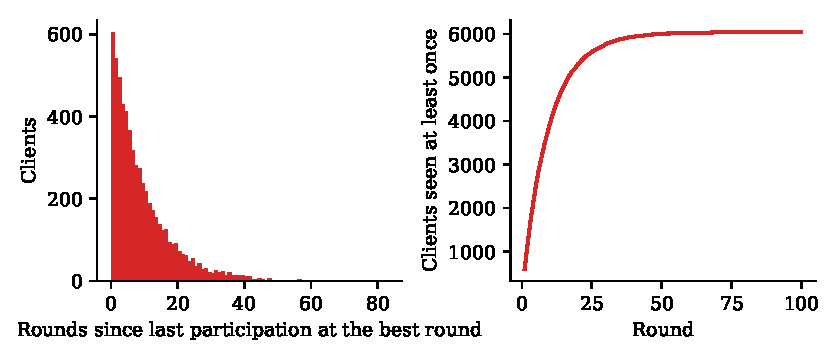
\includegraphics[width=\linewidth]{figures/fig_staleness.pdf}
  \caption{Left: rounds since the last participation of each client at the best round of the
  PFedRec run (\RunPfedrecShort). Right: cumulative number of distinct clients that have
  participated at least once, by round.}
  \label{fig:staleness}
\end{figure}

\section{Statistical Analysis}
\label{sec:setup-stats}

Every comparison between two scoring conditions on the same model, or between two methods, is a
paired comparison over users: $d_u = m_u^{A} - m_u^{B}$ for the per-user metric $m$. The
registered procedure, implemented once and reused for every experiment, reports:
\begin{itemize}[leftmargin=2em]
  \item the mean difference with a 95\% bootstrap confidence interval (10\,000 resamples,
        seed \Seed) \cite{efron1993bootstrap};
  \item the Wilcoxon signed-rank test \cite{wilcoxon1945} with the one-sided hypothesis
        registered for the experiment as primary, the two-sided $p$ as a check, and the
        rank-biserial correlation $r = (W^+ - W^-)/(W^+ + W^-)$ as effect size;
  \item zero differences handled by discarding them (the standard \code{wilcox} rule) in the
        primary test and by Pratt's rule \cite{pratt1959} as a registered sensitivity check,
        because in these experiments most users have $d_u = 0$ exactly;
  \item Holm's correction \cite{holm1979} across the cells of one experiment.
\end{itemize}
The tests describe variability across users for one trained model; they do not describe
variability across random seeds. When the mean and the rank test disagree, as happens when a
few users lose everything while many gain a little, both are reported and the mechanism is
stated (Section~\ref{sec:res-pfedrec}). \pending{paired tests across the four methods require
per-user scores for the Baseline, Personalized and Adaptive runs, which need the re-scoring
adapters for those modules and the runs' saved parameters}.

\section{Pre-registration Practice}
\label{sec:setup-prereg}

From November 2026 every experiment whose number reaches this thesis was registered before it
was run: a README in the result directory fixes the inputs with their hashes, the protocol, the
grid, the statistics, the trust checks that abort the run, numeric predictions, and the rule by
which the result will be reported; a fill-only result file is completed after the run and the
README is not edited afterwards except in a dated changelog. Appendix~\ref{app:posttune}
reproduces the predictions of the post-tuning experiment and their outcome, including the one
that was refuted.

\section{Compute}
\label{sec:setup-compute}

Each federated run took between \RunPfedrecHours{} and \RunPersonalizedHours{} hours of
wall-clock time on one GPU (Table~\ref{tab:runs}). The offline re-scoring of one variant over
all \DsUsers{} users takes seconds on a CPU; the four-cell post-tuning experiment took
\PtElapsedSec{} s. All analysis in Chapters~\ref{ch:results} and~\ref{ch:discussion} is
therefore reproducible without a GPU from the committed result files.
